\documentclass[12pt]{article}
\usepackage[utf8]{inputenc}
\usepackage{graphicx} %package to manage images



\title{ResearchTools Hw1}
\author{Ryan Hill}
\date{September 14, 2018}


\begin{document}
\maketitle
\begin{abstract}
    This is an abstract. In my experience, abstracts usually take longer to write than one would think. One may say, oh, it's just an easy abstract that describes the important aspects of your paper. Then, you find your self spending hours on a stupid little abstract, that seems to have more importance than the paper it is describing. This time could be better spent training as a solider of the Galactic Empire, but no I'm just a lonely Galactic Empire scientist, who does believe in the force.
\end{abstract}

\section{Introduction}
\begin{figure}
\caption{The various Deathstars}
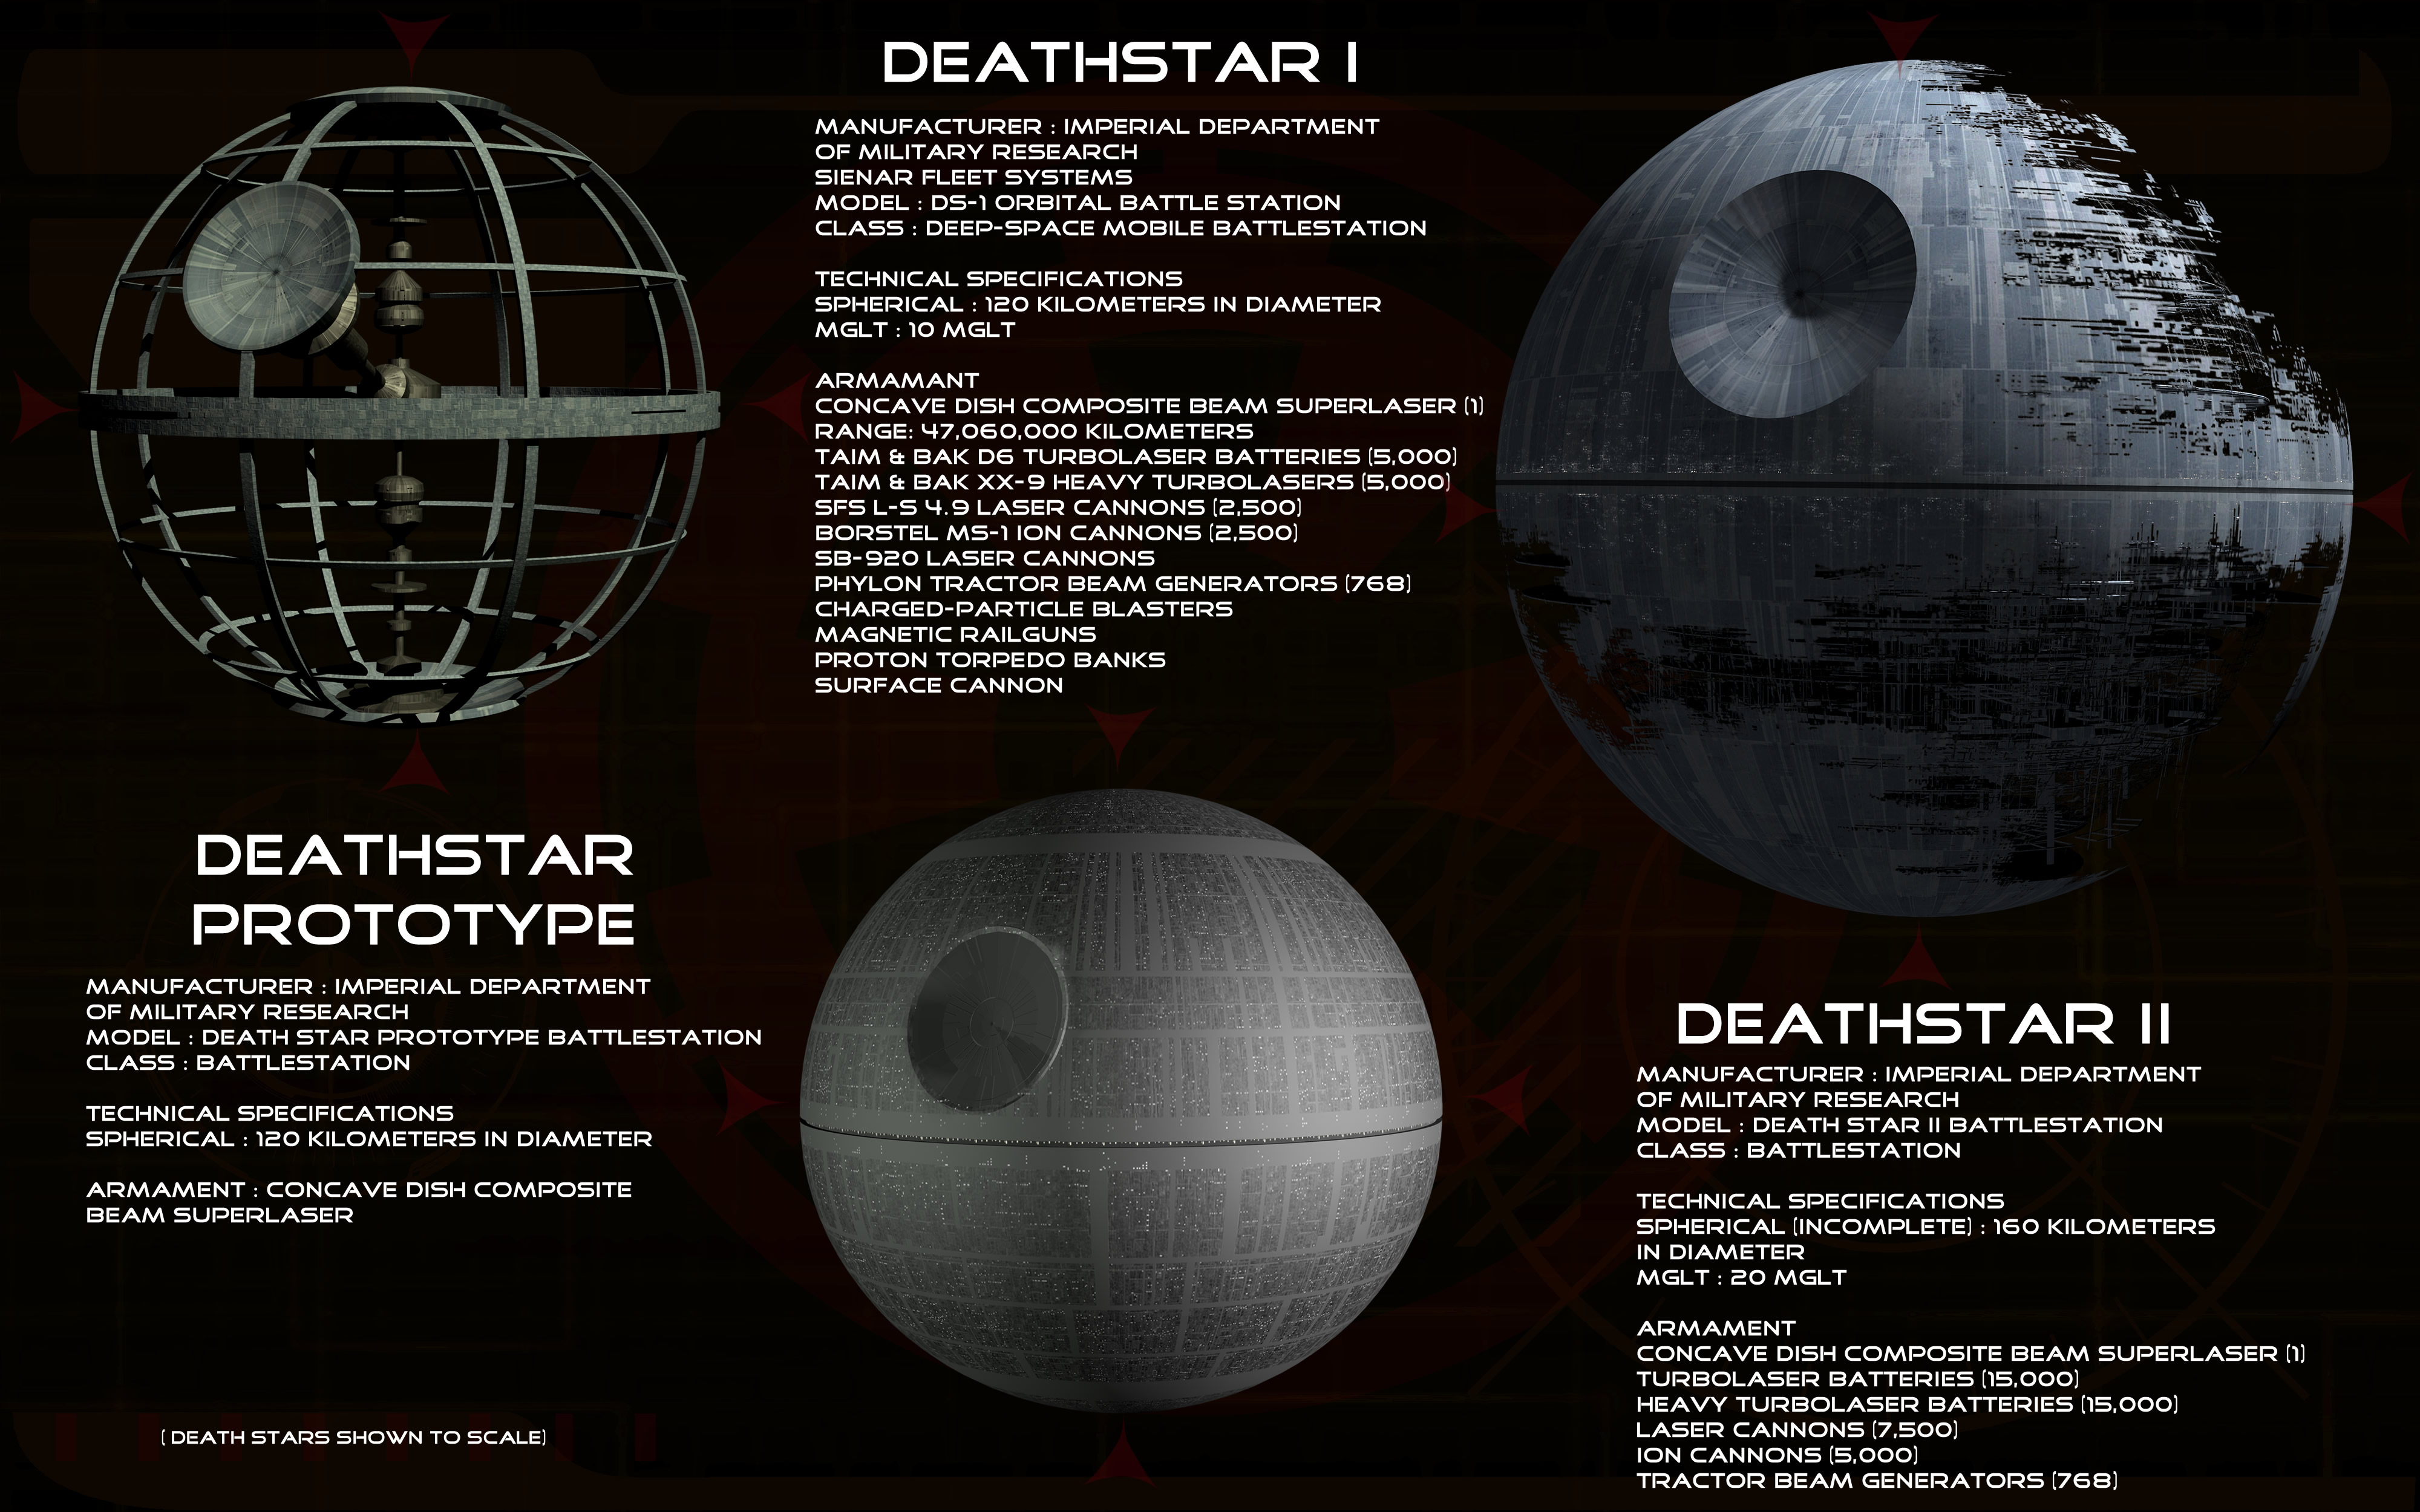
\includegraphics[scale=.1]{./Deathstar.jpg}
\label{DeathStar}
\end{figure}


\paragraph{}
The Galactic Empire, more recently known as the First Order, has ignored the great wisdom of one of the greatest sith Lords, Lord Vader. Lord Vader, predicted the failure of each death star that was built and lobbied for the better use of the Empire's resources. The various sizes of the death stars can be seen in figure \ref{DeathStar}. 

\paragraph{}
Some of the most well known failures of the Galactic Empire are listed in table \ref{1}. I purpose that we use our resources to design a weapon that harness the strength of the force, as was the vision of Lord Vader.

\paragraph{}
\begin{table}
\centering
\label{1}
\caption{The Failures of the Galactic Empire}
\begin{tabular}{|l|l|} 
\hline
1 & Deathstar 1     \\ 
\hline
2 & Deathstar 2     \\ 
\hline
3 & Base on Scarif  \\
\hline
\end{tabular}
\end{table}


\section{Experiments}
    \subsection{Experiment 1}
    \paragraph{}
    In experiment number 1, we see that equation 1 tells us how much resources we are wasting. Building non-force enabled weapons waste the resources of the Galactic Empire on large weapons, such as, the death star.
    
	\paragraph{}
	\begin{equation}
	\label{eq:1}
	f(x,y)=\sqrt{x^2-y^2}
	\end{equation}
	
	
	\paragraph{}
	Using Sith force math, from equation \ref{eq:1} we arrive at
	\large $g_{inv}=\frac{1}{x^2 + y^2}$
    \normalsize which tells us something about the force.
    
    \subsection{Experiment 2}
    \paragraph{}
	This is another force paragraph, which is like a force ghost, but for papers. Equation 2 tells is something about the force, but who knows what exactly.    
    
    \begin{equation}
	\sum_{i=0}^n n^2
	\end{equation}
    	
    \paragraph{}
    This paragraph is about equation 3, which is just an array.
    \begin{equation}
\left(\begin{array}{ccc}1 & 2 & 3\\ 4 & 5 & 6\\ 7 & 8 & 9\end{array}\right) 
	\end{equation}
	
	\paragraph{}
	The final paragraph about a force equation is equation 4.
	    \begin{equation}
a_0 \frac{1}{
a_1+ \frac{1}{
a_2+ \frac{1}{
\ddots \, + \frac{1}{
a_n
}}}}
	\end{equation}
	
	
\section{Conclusion}
\paragraph{}
One can see clearly from equation \ref{eq:1}, that we must stop wasting the resources of the Galactic Empire.

\paragraph{}
As Galactic Empire engineers and scientist, it is up to us to stop the rebel scum by creating weapons that use the force. We may still be able to secure the legacy of Lord Vader's brilliance.  

\end{document}